\section{Lecture One}
\begin{itemize}
    \item Groups are everywhere in mathematics and nature in one of two forms:
    \begin{itemize}
        \item as groups of symmetries
        \item as groups of ``numbers'' or quantities
    \end{itemize}
    \item We will call a subset $F \subseteq \mathbb{R}^n$ a \textbf{figure} in $\mathbb{R}^n$ when we consider $F$ not just as a set, but as a set together with the structure of its distance functions:
    \begin{equation}
        d: F \times F \mapsto \mathbb{R}_{\ge 0},\quad d(x,y) = \lVert x-y \rVert
    \end{equation}
    A figure is then defined as the pair $(F,d)$.
    \begin{definition}
        A \textbf{symmetry} of a figure $F \subseteq \mathbb{R}^n$ is a bijection $\sigma: F \mapsto F$ such that $\sigma$ and $\sigma^{-1}$ preserve distances:
        \begin{align}
            \forall x,y, \in F,\quad& d(\sigma(x),\sigma(y))=d(x,y) \\ 
            \iff & d(\sigma^{-1}(x), \sigma^{-1}(y)) = d(x,y)
        \end{align}
        Therefore:
        \begin{equation}
            \text{Sym}(F) \equiv \{\sigma: F\to F | \sigma\text{ is a symmetry}\}
        \end{equation}
    \end{definition}
    \item For example, any point, line, shape, or form is a figure. However, we are only interested in figures that have interesting symmetries.
    \begin{example}
        Let $F$ be a square in $\mathbb{R}^2$. There are four different lines of reflections:
        \begin{center}
            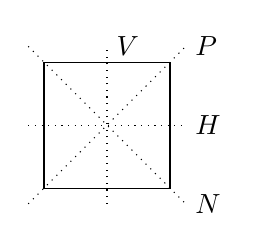
\begin{tikzpicture}
                \draw[] (0.2,0.2) -- (1.8,0.2) -- (1.8,1.8) -- (0.2,1.8) -- cycle;
                \draw[dotted] (1,0) -- (1,2) node[right] {$V$};
                \draw[dotted] (0,1) -- (2,1) node[right] {$H$};
                \draw[dotted] (0,0) -- (2,2) node[right] {$P$};
                \draw[dotted] (0,2) -- (2,0) node[right] {$N$};
            \end{tikzpicture}
        \end{center}
        and there are three rotations: $R_1$, $R_2$, and $R_3$, which represent $90^\circ$, $180^\circ$, and $270^\circ$ clockwise rotations. $I$ represents the identity transformation (do nothing).
        \vspace{2mm}

        We can combine symmetries. For example, what is $R_1 \circ V$? To do so, we can label the vertices:
        \begin{center}
            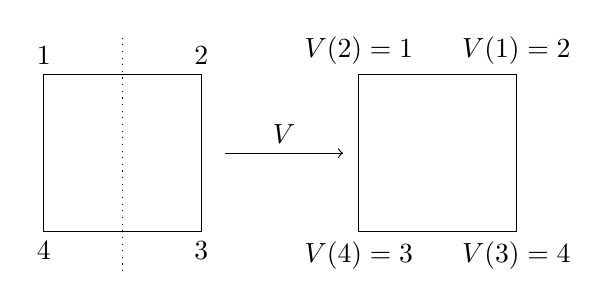
\begin{tikzpicture}
            \begin{scope}
                \draw[] (0,2) node[above]{$1$}
                -- (2,2) node[above]{$2$}
                -- (2,0) node[below]{$3$}
                -- (0,0) node[below]{$4$} -- cycle;
                \draw[dotted] (1,-0.5) -- (1,2.5);
            \end{scope}
            \begin{scope}[xshift=4cm]
                \draw[] (0,2) node[above]{$V(2)=1$}
                -- (2,2) node[above]{$V(1)=2$}
                -- (2,0) node[below]{$V(3)=4$}
                -- (0,0) node[below]{$V(4)=3$} -- cycle;
            \end{scope}
            \draw[->] (2.3,1) -- (3.8,1) node[midway, above] {$V$};
            \end{tikzpicture}
        \end{center}
        \begin{center}
            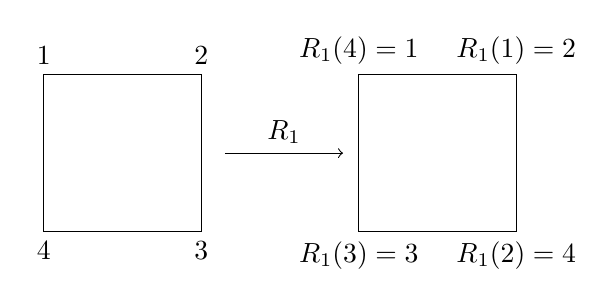
\begin{tikzpicture}
                \begin{scope}
                \draw[] (0,2) node[above]{$1$}
                -- (2,2) node[above]{$2$}
                -- (2,0) node[below]{$3$}
                -- (0,0) node[below]{$4$} -- cycle;
                \end{scope}
            \begin{scope}[xshift=4cm]
                \draw[] (0,2) node[above]{$R_1(4)=1$}
                -- (2,2) node[above]{$R_1(1)=2$}
                -- (2,0) node[below]{$R_1(2)=4$}
                -- (0,0) node[below]{$R_1(3)=3$} -- cycle;
            \end{scope}
            \draw[->] (2.3,1) -- (3.8,1) node[midway, above] {$R_1$};

            \end{tikzpicture}
            
        \end{center}
        Applying the computations:
        \begin{align}
            (R_1 \circ V)(1) &= R_1(V(1)) = R_1(2) = 3 \\ 
            (R_1 \circ V)(2) &= R_1(V(2)) = R_1(1) = 2 \\ 
            (R_1 \circ V)(3) &= 1 \\ 
            (R_1 \circ V)(4) &= 4
        \end{align}
        Check that $V \circ R_1 = N$. Also notice that these operations are not commutative: $R_1 \circ V \neq V \circ R_1$.
    \end{example}
    \item In the above example, how are we sure that these are all of the symmetries of a square? To answer this, we will need the following facts:
    \begin{enumerate}
        \item A symmetry maps vertices to vertices. The vertices are the points of the square that are furthest from the center.
        \item Symmetries map adjacent vertices tto adjacent vertices. If $x$, $y$ are adjacent vertices, then $\sigma(x)$, $\sigma(y)$ are vertices, and $d(\sigma(x),\sigma(y))=d(x,y)=\text{side length}$.
        \item A symmetry $\sigma$ is completely determined by $(\sigma(1), \sigma(2))$. For example, suppose we have the symmetry $\sigma$ on a square such that:
        \begin{center}
            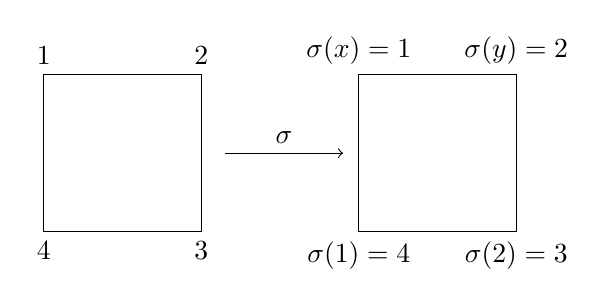
\begin{tikzpicture}
            \begin{scope}
                \draw[] (0,2) node[above]{$1$}
                -- (2,2) node[above]{$2$}
                -- (2,0) node[below]{$3$}
                -- (0,0) node[below]{$4$} -- cycle;
            \end{scope}
            % \begin{scope}[xshift=3cm, yshift=1cm]
            %     \node[] (0,0) {$\longrightarrow$};
            % \end{scope}
            \begin{scope}[xshift=4cm]
                \draw[] (0,2) node[above]{$\sigma(x)=1$}
                -- (2,2) node[above]{$\sigma(y)=2$}
                -- (2,0) node[below]{$\sigma(2)=3$}
                -- (0,0) node[below]{$\sigma(1)=4$} -- cycle;
            \end{scope}
            \draw[->] (2.3,1) -- (3.8,1) node[midway, above] {$\sigma$};
            \end{tikzpicture}
        \end{center}
        From this, we know that we  must have $y=3$, from fact 1, as well as $x=4$.
        \item For all $x,y\in\{1,2,3,4\}$ such that $x$ is adjacent to $y$, $\exists!$ symmetry $\sigma$ of the square such that:
        \begin{equation}
            (\sigma(1), \sigma(2)) = (x,y)
        \end{equation}
    \end{enumerate}
    By the above facts, we must count the ordered pairs $(x,y)$ such that $x,y \in \{1,2,3,4\}$ and $x$ is adjacent to $y$:
    \begin{itemize}
        \item There are $4$ choices for $x$.
        \item For each choice of $x$, there are two choices of $y$. Therefore, there are $4\times 2 = 8$ symmetries.
    \end{itemize}
    Since we listed $8$ different symmetries of a square, we have therefore defined all of them.
\end{itemize}